\chapter{ \label{appendix:compensation} Compensation: accounting for fluorescent signal crosstalk in flow cytometry}

\begin{figure} [ht]
\begin{center}
   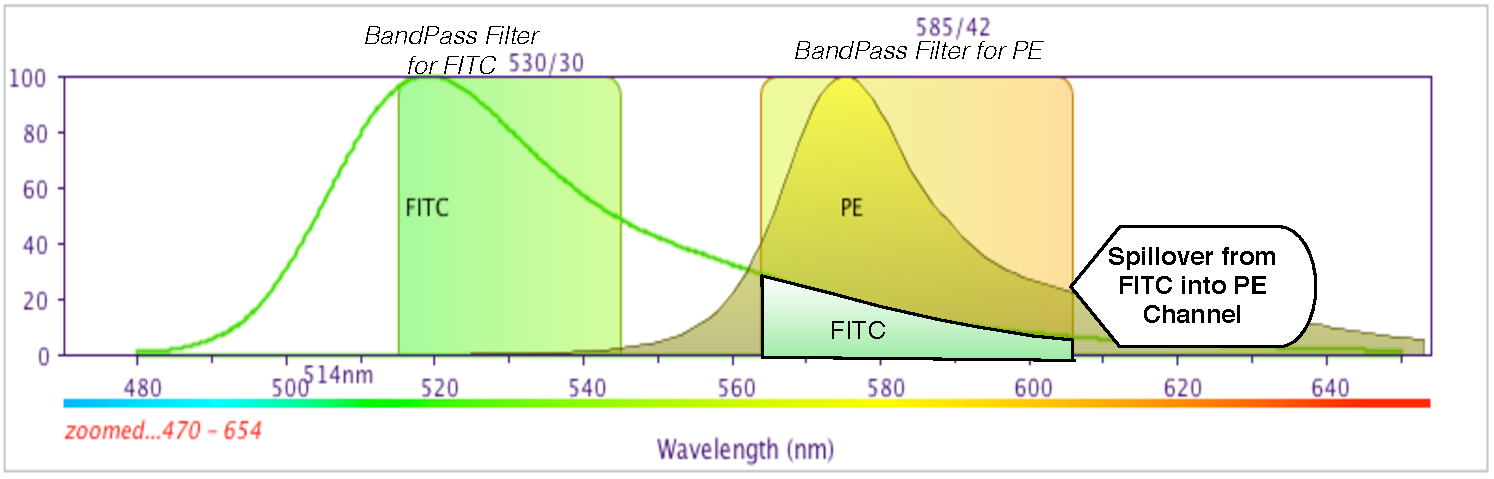
\includegraphics[scale=0.6]{introduction2/figures/spillover.pdf}
\end{center}
\mycaption{figure:spillover}
{ Leaking of signal from FITC fluorochrome into PE detector.}
{
  \small{Created using: \url{http://www.bdbiosciences.com/research/multicolor/spectrum_viewer/}}
}
\end{figure}

\begin{table}[ht]
\begin{center}
\begin{tabular}{rrrrrrr}
  \hline
%\backslashbox{Signal}{Detector} & Alexa-488 & PE-Cy7 & APC & PE & Alexa-700 & Pacific Blue \\ 
\backslashbox{Signal}{Detector} & PMT 1 & PMT 2 & PMT 3 & PMT 4 & PMT 5 & PMT 6 \\ 
  \hline
Alexa-488    & 100 &   0 &   0 &  16 &   0 &   0 \\
PE-Cy7       &   0 & 100 &   0 &   1 &   2 &   0 \\
APC          &   0 &   0 & 100 &   0 &  30 &   0 \\
PE           &   2 &   1 &   0 & 100 &   0 &   0 \\
Alexa-700    &   0 &   1 &   2 &   0 & 100 &   0 \\
Pacific Blue &   0 &   0 &   0 &   0 &   0 & 100 \\
   \hline
\end{tabular}
\end{center}
\mycaption{table:spillover}
{ Spillover matrix of the fluorochomes used by \citet{Dendrou:2009dv} obtained using single colour beads. }
{
Each entry is the percentage of the emitted fluorochrome signal (row) picked up by a detector (column).
The rows represent the fluorochomes and the columns are the PMT detectors.
Each detector is tuned to capture the intensity of a single fluorochrome (diagonal entries).
Spillover occurs when certain fluorochromes are detectable by more than one detector (non-zero terms off the diagonal).
Notice that there is non-negligeable spillover (\SI{30}{\percent}) of APC into PMT 5, the detector meant for Alexa-700.
}
\end{table}


%As we delve deeper into the lymphocyte subsets more fluorochromes are needed to further distinguish between different classes \citep{Perfetto:2004cy}.
%However when adding more and more fluorochromes, overlap of emission spectra becomes unavoidable.
%This implies that the intensity signal captured in a given detector is no longer originating from one single fluorochrome but is actually a combined signal emanating from multiple fluorochromes \citep{Roederer:2001vi}.
%To account and correct for this, the overlap needs to be assessed by evaluating the pairwise contribution of the signal of one fluorochrome to that of an other.
%These pairwise values can then be summarised in what is known as a spillover or compensation matrix (Table~\ref{table:spillover}).
%By subtracting the spillover values to the mixed intensity one can then recover the original intensity.
%This compensation step is usually performed after all the data from an experiment has been collected before commencing analysis.

As we delve deeper into the lymphocyte subsets more fluorochromes are needed to further distinguish between different classes \citep{Perfetto:2004cy}.
However when adding more and more fluorochromes, overlap of emission spectra becomes unavoidable \citep{Roederer:2001vi}.
%This implies that the intensity signal captured in a given detector is no longer originating from one single fluorochrome but is actually a combined signal emanating from multiple fluorochromes \citep{Roederer:2001vi}.
This implies that the intensity signal measured in one detector is in fact a mixture of signals from other flurochromes which spillover across detectors (Figure~\ref{figure:spillover}).
The deconvolution of this signal is a process known as compensation.
The matrix solution is known as the spillover matrix and is usually a square matrix with as many rows as there are fluorochromes and columns as there are detectors
%if there as many dyes as there are detectors 
(Table~\ref{table:spillover}).
To calculate the spillover matrix single coloured beads are used. 
The pairwise contribution of a fluorochrome to a non-specific channel is then summarised in a compensation matrix.
%To account and correct for this, the overlap needs to be assessed by evaluating the pairwise contribution of the signal of one fluorochrome to that of an other.
%These pairwise values can then be summarised in what is known as a spillover or compensation matrix (Table\ref{table:spillover}).

%This phenomenon is known as spectral spillover.

By subtracting the spillover values from the mixed intensity one can then recover the original intensity.

This compensation step is usually performed after all the data from an experiment has been collected before commencing analysis.


